%% LyX 2.3.5.2 created this file.  For more info, see http://www.lyx.org/.
%% Do not edit unless you really know what you are doing.
\documentclass[french]{article}
\usepackage[T1]{fontenc}
\usepackage[utf8]{inputenc}
\usepackage{geometry}
\usepackage{graphicx}
\graphicspath{ {./images/} }
\geometry{verbose,tmargin=2cm,bmargin=2cm,lmargin=2.5cm,rmargin=2.5cm,headheight=1cm,headsep=1cm,footskip=1cm}
\setlength{\parskip}{\medskipamount}
\setlength{\parindent}{0pt}

\makeatletter
%%%%%%%%%%%%%%%%%%%%%%%%%%%%%% User specified LaTeX commands.
\usepackage{listings}
\usepackage{xcolor}
\usepackage[utf8]{inputenc}

\makeatother

\usepackage{babel}
\makeatletter
\addto\extrasfrench{%
   \providecommand{\og}{\leavevmode\flqq~}%
   \providecommand{\fg}{\ifdim\lastskip>\z@\unskip\fi~\frqq}%
}

\makeatother
\begin{document}
\title{IFT 712 - Techniques d'apprentissage\\
Projet de session}
\author{Étienne Ameye\\
Yanni Mansour\\
Djibril Sene}
\date{Lundi, 11 décembre 2023}
\maketitle

\pagebreak

\tableofcontents
\pagebreak

\section{Méthodologie}

\subsection{Structure du projet}

\subsection{Jeu de données}

\subsection{Méthodes d'évaluation}

\section{Évaluation des résultats}

\subsection{Classifieur KNN}

\subsection{Régression logistique}

Le deuxième modèle que nous avons choisi d’utiliser est le modèle de régression logistique. Il s’agit une technique de modélisation statistique utilisée normalement pour prédire la probabilité d'appartenance à une classe binaire en fonction de variables indépendantes. Elle est couramment utilisée dans les problèmes de classification, tels que la prédiction de la catégorie d'appartenance d'un élément parmi deux classes distinctes.\\ 
\par
Cependant, notre problème comporte plus de deux classes, mais il est possible d’utiliser des approches adaptant la régression logistique à un modèle multi-classes. On peut en effet utiliser une approche dite "one-vs-rest" (OvR) ou multinomiale. Ces 2 approches sont disponibles via le paramètre multi\_class de sklearn.LogisticRegression. La différence principale entre ces 2 méthodes est qu’en OvR, un modèle de régression est créé pour chaque classe par rapport aux autres classes combinées alors qu’avec la méthode multinomiale, toutes les classes sont gérées en même temps. Dans le cadre du modèle que nous avons créé, après avoir fait des tests de performances en changeant seulement la valeur du paramètre multi\_class, nous n’avons pas observé de différences remarquables de performances, nous avons donc laissé le paramètre en automatique, soit en OvR. 
\par
Les hyperparamètres que nous avons choisit d’optimiser sont les suivants : 
- La régularisation, contrôlée par le paramètre C. Plus la valeur de C est petite, plus la régularisation est forte.
- Le choix de la norme de pénalité, régulée par le paramètre penalty, qui peut être "l1" (Lasso) ou "l2" (Ridge).
- Le type de solveur utilisé pour l'optimisation, spécifié par le paramètre solver, il peut être de type ‘liblinear’, ‘newton-cg’, ‘sag’ ou ‘saga’. Il détermine l’algorithme utilisé pour le problème d’optimisation du modèle. 
\par
Pour le type de solveur et la norme de pénalité, nous avons fait le choix de tous les tester dans la recherche d’hyperparamètres de notre modèle. Par contre, pour la régularisation, il s’agit d’une valeur numérique , qui peut prendre n’importe quelle valeur positive, il a donc fallu faire un choix sur la plage de données à tester. La détermination de cette plage s’est faite par tâtonnements, en testant différentes valeurs de C pour la recherche d’hyperparamètres. Nous avons commencé par des valeurs proches de 10, pour arriver à obtenir des scores de performances satisfaisants aux alentour de C = 100. Au final, la plage de valeur testée est [60 ; 160], avec un écart de 20 entre chaque valeur. Nous avons choisi de nous limiter le nombre de valeurs testées et leur amplitude afin d’avoir des temps de calculs raisonnables.\\
\par
Après avoir effectué la recherche des meilleurs hyperparamètres, la meilleure combinaison pour l’entraînement obtenue est la suivante : C = 160, penalty = ‘l2’ et solver  = ‘liblinear’, avec un score de précision de 0.912.\\
Dans un premier temps, on remarque que la valeur de C est la plus élevée parmi celles présentes dans l’intervalle de recherche. Cela confirme les observations faites précédemment lors du processus de recherche des valeurs des hyperparamètres à tester. Sachant que C est l’inverse de la force de régularisation, cela signifie que moins la régularisation est forte, mieux notre modèle performe sur les données d’entraînement. Afin de constater l’importance de cet hyperparamètre par rapport aux autres, nous traçons les courbes représentant les différentes combinaisons d’hyperparamètres testés :
\begin{figure}
    \centering
    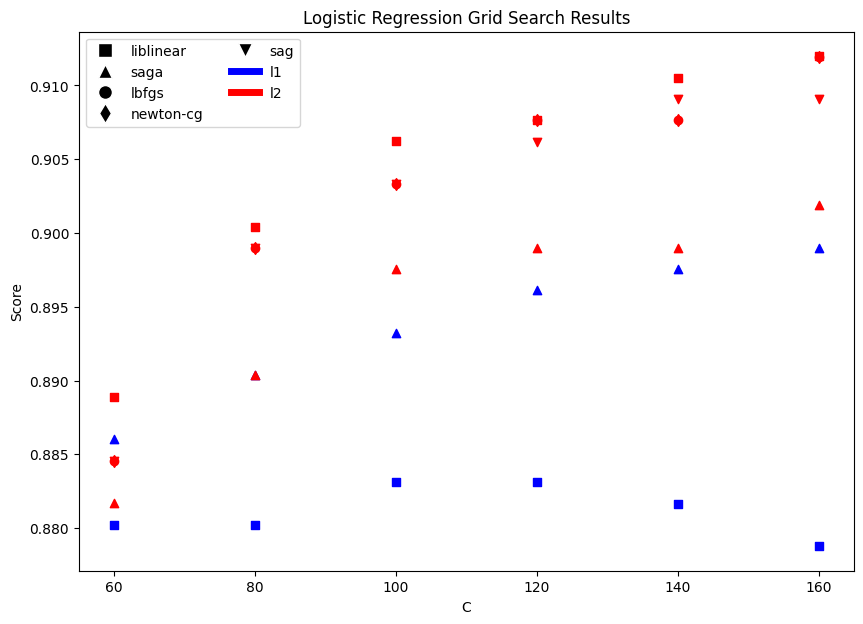
\includegraphics[width=0.7\linewidth]{courbe_lr.png}
    \caption{Enter Caption}
    \label{fig:enter-label}
\end{figure}

Dans un premier temps, il est important de noter que toutes les combinaisons possibles d’hyperparamètres ne sont pas présentes. Cela est dû au fait que certains solvers ne sont compatibles qu’avec certaines pénalités, comme newton-cg qui n’est compatible qu’avec une pénalité l2.
\par
 Ensuite, nous observons clairement une augmentation nette du score plus la valeur de C est élevée, pour toutes les combinaisons d’hyperparamètres, hormis quand le solver est liblinear et la pénalité l1. En outre, le choix de la pénalité a également un impact important sur les performances, les courbes en rouges, représentant la pénalité l2 sont au-dessus des bleues représentant l1. Cela peut s’expliquer par plusieurs raisons. La pénalité l2 est meilleure lorsque les données possèdent des caractéristiques corrélées,  ce qui est le cas pour nos données où les 3 caractéristiques sont divisées en 64 sous caractéristiques. De plus , la pénalité l2 est souvent utilisée dans les cas où le nombre d’observations est limité comparé au nombre de classes, correspondant bien à notre jeu de données.
 \par
Enfin, pour les solvers couplés à la pénalité l2, nous observons que liblinear, lbfgs, sag et newton-cg obtiennent des résultats assez similaires, et avec saga légèrement en-dessous. Le solver liblinear reste tout de même le plus performant peut importe la valeur de C, mais avec une marge de moins en moins grande plus C augmente. Pour notre modèle, le choix du solver n’a donc pas d’impact significatif sur les performances par rapport aux deux autres hyperparamètres. 
\par
Pour réellement mesurer les performances du meilleur modèle sur l’ensemble d’entraînement, nous l’évaluons sur un ensemble de test composé de données que le modèle n’a jamais rencontré. Voici les valeurs moyennes des métriques de performances obtenues pour chaque classe : \\ 
\par
- precision : 93.822\%$ \pm 14.766\%$ \\
- recall    : 92.929\%$ \pm 16.682\%$ \\
- f1\_score  : 92.350\%$ \pm 13.945\%$ \\
\par
Nous traçons également les boxplots correspondants :
\begin{figure}
    \centering
    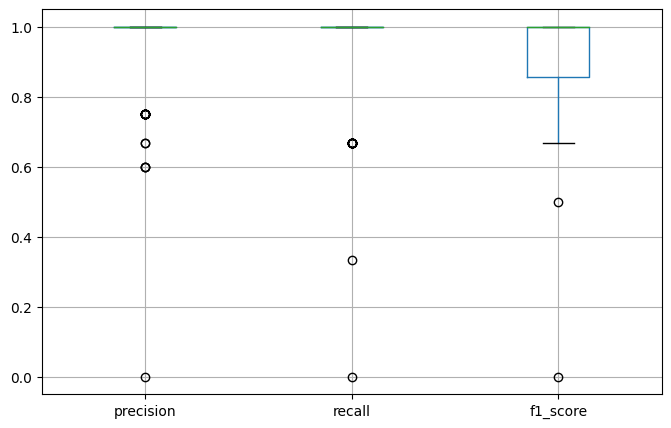
\includegraphics[width=0.7\linewidth]{boxplot_lr.png}
    \caption{Enter Caption}
    \label{fig:enter-label}
\end{figure}
\par
D’abord, on remarque que les valeurs des 3 métriques de performances sont très élevées, avec $93,8\%$ de précision et un recall et f1\_score aux alentours de $92,3\%$. 
Comme on peut le voir dans les boxplots, les prédictions sont correctes pour la grande majorité des classes, avec seulement très peu de valeurs aberrantes (outliers). On peut cependant observer que le boxplot du f1\_score est un peu plus étendu, indiquant quelques erreurs de prédictions, mais rien de critique, la médiane étant aux alentours de 0.9. 
\par
Il existe cependant des classes pour lesquelles le modèle a moins bien performé. Au total, 34 classes sur les 99 on un f1\_score non parfait, c’est-à-dire différent de 1. Cela n’est absolument pas alarmant sur les performances de notre modèle, mais indique que des points d’améliorations subsistent pour encore augmenter les performances de celui-ci.
\par
Enfin, nous dressons la matrice de confusion qui montre toutes les erreurs de prédictions, en affichant les couples de classes où une classe prédite était différente de la classe réelle, avec le nombre d’occurrences.

\begin{figure}
    \centering
    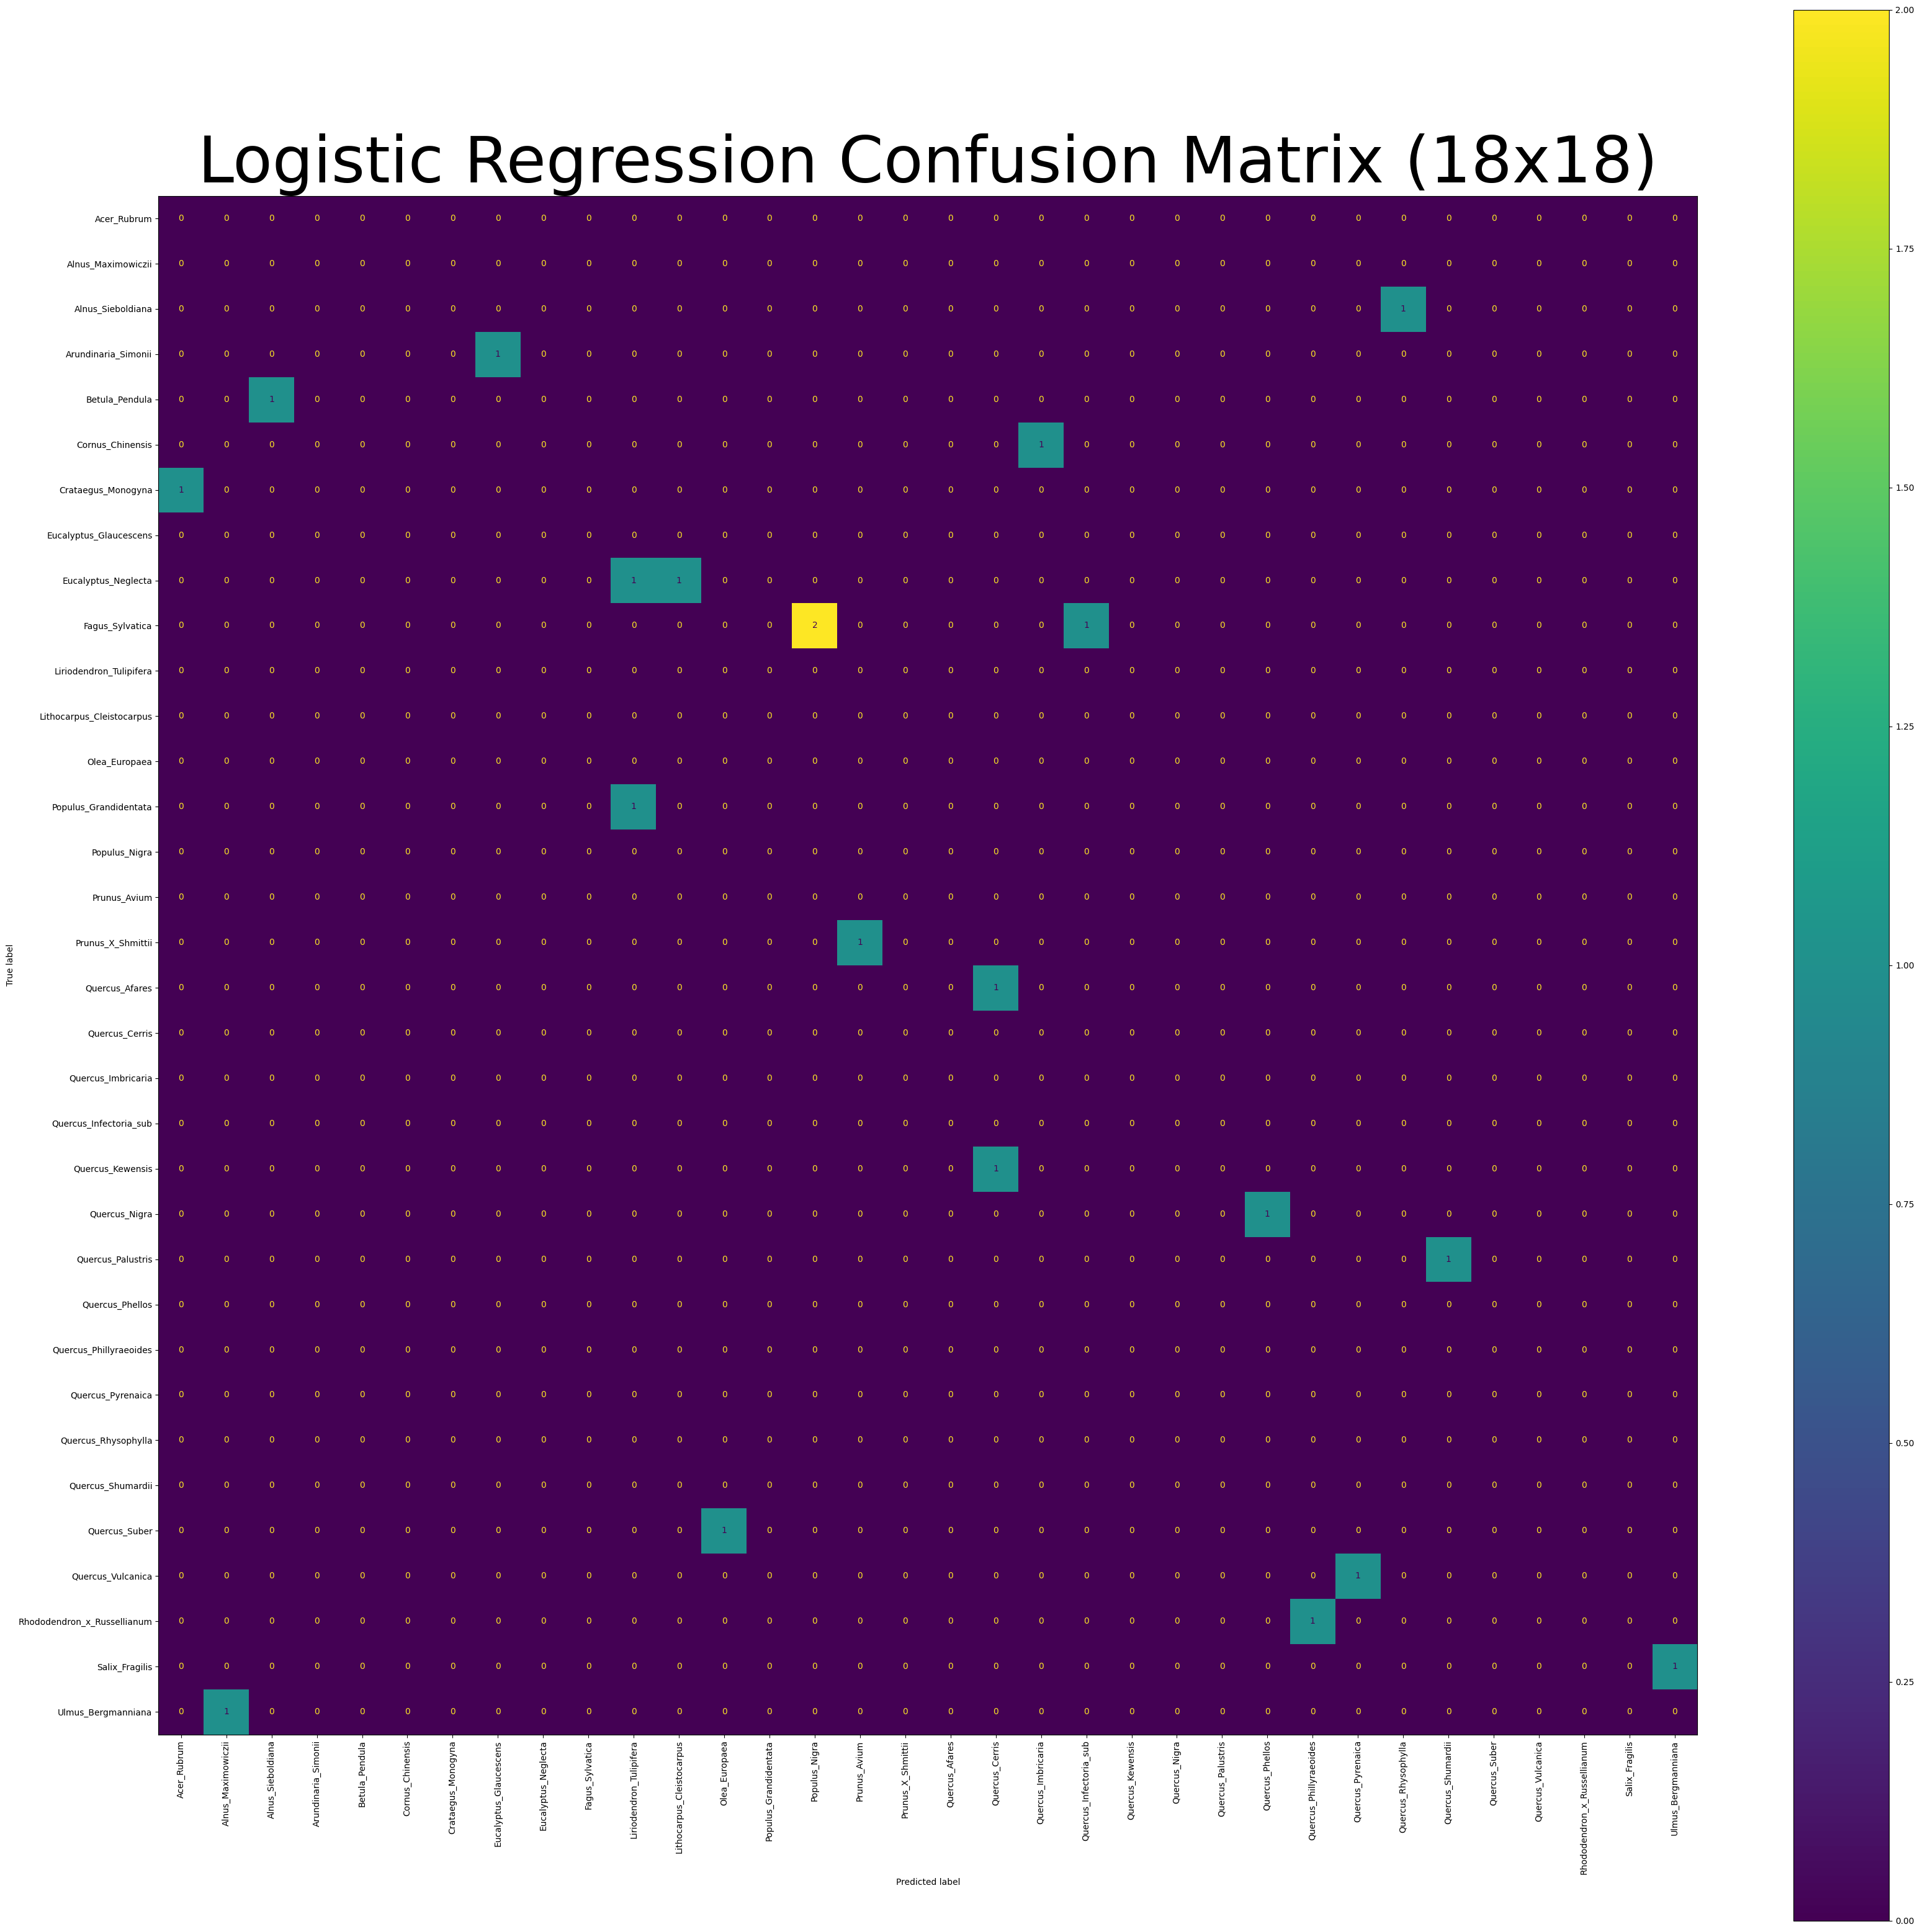
\includegraphics[width=0.7\linewidth]{matrix_lr.png}
    \caption{Enter Caption}
    \label{fig:enter-label}
\end{figure}
\par
Comme observé précédemment via les métriques de performances, nous voyons que les erreurs de prédictions sont rares et ne sont pas concentrées sur une classe en particulier. On peut seulement relever le fait que la feuille de type Falgus\_Sylvatica est la seule classe a mal avoir été prédite à 3 reprises.\\[2\baselineskip]



{\textbf{\Large Conclusion :}}

Malgré son origine binaire, le modèle de régression logistique s’est révélé plutôt performant pour résoudre notre problème de classification. Nous avons en ce sens adapté la régression logistique à un modèle multi-classes en utilisant l'approche OvR.

Les meilleurs hyperparamètres trouvés sont la régularisation C = 160, la norme de pénalité = 'l2'et le type de solveur 'liblinear', avec un score de précision de $91.2\%$ sur les données d’entraînement, et des métriques de performance allant de 92 à $94\%$ sur les données de test. 

L'analyse des performances en fonction de la régularisation (C) a révélé que des valeurs plus élevées de C ( donc moins de régularisation) ont conduit à de meilleures performances sur l'ensemble d'entraînement. La pénalité l2 a également montré des performances supérieures à la pénalité l1, probablement en raison de la nature de nos données avec des caractéristiques corrélées. Enfin, le choix du solveur n’a pas eu d’impact significatif sur les performances, particulièrement pour des valeurs de C élevées.

Les boxplots ont montré une bonne cohérence des performances avec peu de valeurs aberrantes et a matrice de confusion a identifié quelques erreurs de prédictions, mais dans l'ensemble, le modèle a bien généralisé sur l'ensemble des classes. Il y a des opportunités d'amélioration spécifiques pour certaines classes où le modèle a rencontré plus de difficultés.

En conclusion, la régression logistique s'est révélée être une approche robuste pour notre problème de classification de feuilles à 99 classes, offrant de bonnes performances sur l'ensemble de test. Des ajustements futurs pourraient inclure des stratégies spécifiques pour les classes présentant des difficultés, ainsi que l'optimisation plus poussée d’autres hyperparamètres en acceptant des temps de calculs plus élevés, pour une comparaison approfondie des performances avec le modèle actuel.


\subsection{Machine à vecteurs de support}

\subsection{Classifieur AdaBoost}

\subsection{Arbre de décisions}

\subsection{Forêt aléatoire}

\section{Conclusion}
\end{document}
